\chapter{1877 The 'G' Red Overprints}    

During April 1877 five values of the current Cape of Good Hope stamps were  overprinted in red and one (the 1d) overprinted in black with a large capital 'G'. These stamps are referred to as the red overprints, despite the exceptional use of black ink for the 1d. value. Of course it did not make much sense to have the 1d. overprinted in red, as it would be very difficult to distinguish it from the background of the carmine-red colour of the postage stamp. Six values of the Cape stamps were overprinted as follows:

\begin{tabular}{ll}$\frac{1}{2}$d. grey-black & 6d. violet\\
1d. carmine-red & 1s. green\\
4d. blue (with outer frame line) &5s. orange-yellow\\
4d. blue (without outer frame line)\\
\end{tabular}

All stamps are perforated 14 and watermarked Crown over CC.

The issue has been plated by Holmes, based on extending studies by...

\ph[width = .60\textwidth]{../griqualand-west/plate.jpg}{Complete setting as given by Holmes. The asterisk indicates a broken type.}

The overprinting was done very carefully, though one half-sheet of 120 of the 1/- vaue received the overprint inverted. Only Type 1 is catalogued by Stanley Gibbons, but several of the other types also exist. Of these the Royal Collection has types 1a, 2a, and 4, while the Tapling Collection includes Types 1a, 2a, 4 and 6. It seems likely that most of the half-sheet was returned to Cape Town with the remainders in 1880, as a majority of the known inverts have Cape Colony cancellations.

Double overprints exist on the 6d., 1/-, and 5/-, but they are more in the nature of
'jumps' rather than the result of two distinct impresions, and are not of any real importance.

\begin{figure*}

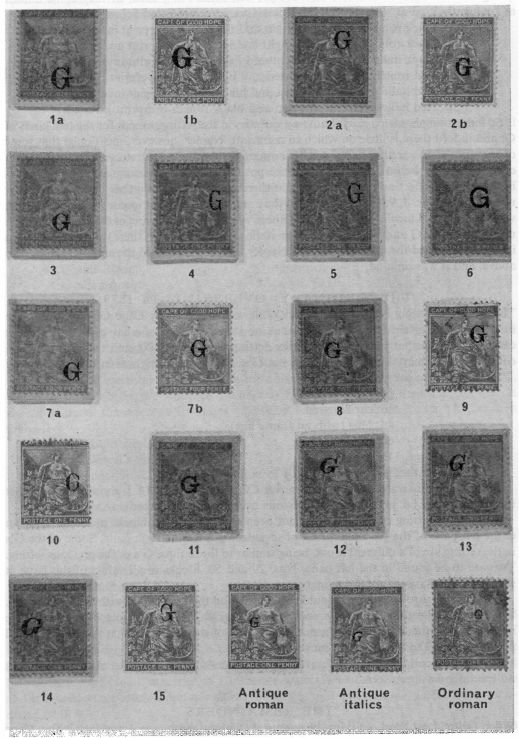
\includegraphics[width=1.0\textwidth]{../griqualand-west/types.jpg}

\caption{The various types as described by Holmes. The image is from his article in the London Philatelist. }
\end{figure*}



\ph[width = .98\textwidth]{../griqualand-west/AC389.jpg}{AC389	1878 watermark Crown CC, 1d carmine-red block of 48 (6x8) with interpanneau margin at right (Somerset House perforator producing 'wing margins'). Overprinted 'G' (types 7 or 9) with each stamp showing an albino impression on the gum, printed onto the reverse, inverted. Two with tears, a few creases and some reinforcing though remarkably fresh mint with many unmounted. A very rare and spectacular multiple. SG 11b, 11d	\pound2,800 }

\ph[width = .30\textwidth]{../griqualand-west/AC630.jpg}{ AC630	1878 4d dull blue without frame lines, with interpanneau margin at left, overprinted 'G' (Type 6) in red. Thinning along edge of interpanneau margin and a few blunt perfs at top, otherwise a very fine mint example in an attractive deep shade. Very scarce. SG 6f	\pound325, rhodesia.co.za}

\ph[width = .95\textwidth]{../griqualand-west/AC633.jpg}{AC633	1877-78 6d deep lilac overprinted 'G' (Type 1a) in red. Horizontal strip of three with interpanneau margin at right. The right stamp with horizontal split at top and the gum somewhat yellowed though a rare and attractive multiple. SG 8a	\pound650. }

\subsubsection{Second Printing}

A number of stamps do not fit in the plating study quoted above. 
                              
                              
\LP{Holmes H.R.}{The Postage Stamps of Griqualand West, Part III}{January 1963}{71:841 LP841.pdf}           

From McGregor dealer's stock, June 2013.
      